\chapter{Results}

This chapter reports the main quantitative and qualitative outcomes of the
project. Final Try 80 test results are intentionally left as placeholders
because the model is still being trained and the final checkpoint has not yet
been frozen.

\section{Experiments and Tests}

Table~\ref{tab:timeline_results} summarizes the most important milestones. The
early rows are not meant as a leaderboard because masking rules and objectives
changed during the project; they document why the next stage was necessary.

\begin{table}[ht]
\centering
\caption{Representative experimental milestones.}
\label{tab:timeline_results}
\begin{tabularx}{\textwidth}{p{2.2cm}>{\raggedright\arraybackslash}X>{\raggedright\arraybackslash}X}
\toprule
Attempt family & Main lesson & Representative result \\
\midrule
Try 1--22   & U-Net/cGAN and decoder fixes; cGAN did not solve physical error. & Try 22 became the clean pre-prior baseline. \\
Try 33--40  & Ground-only masking became mandatory. & Building pixels excluded from loss and metrics. \\
Try 41--50  & Prior plus residual helped LoS but NLoS remained dominant. & Try 42: \SI{19.78}{dB} overall, \SI{3.86}{dB} LoS, \SI{34.47}{dB} NLoS. \\
Try 66      & PMHHNet synthesis with six experts and physical channels. & \SI{9.41}{dB} overall, \SI{3.75}{dB} LoS, \SI{31.48}{dB} NLoS. \\
Try 76      & Distribution-first path-loss modelling. & NLoS pixel-weighted RMSE $\approx$\,\SI{3.34}{dB}. \\
Try 78      & Non-DL calibrated path-loss prior. & \SI{1.92}{dB} overall, \SI{1.75}{dB} LoS, \SI{3.40}{dB} NLoS. \\
Try 79      & Non-DL calibrated spread priors. & \SI{28.10}{ns} delay; \SI{13.74}{\degree} angular. \\
Try 80      & Joint prior-anchored model. & Validation snapshot: \SI{1.77}{dB} path loss; final test pending. \\
\bottomrule
\end{tabularx}
\end{table}

Try 78 is the clearest path-loss breakthrough. The coherent two-ray LoS model
reduced LoS RMSE from roughly \SI{3.95}{dB} with FSPL to
\SI{1.75}{dB}. The final hybrid prior reached \SI{1.9246}{dB} overall under the
pixel-weighted metric.

\section{RMSE evolution and interpretation}

The RMSE history should be read as a sequence of increasingly strict
experiments, not as a perfectly homogeneous leaderboard. The dataset changed,
the building-mask rule became stricter after the early experiments, and later
tries used city-holdout discipline more consistently. Nevertheless, the
representative values in Table~\ref{tab:rmse_evolution} show the real
direction of the project: from direct image regression, to prior-guided
residual learning, to frozen calibrated priors and finally to the joint Try 80
model.

\begin{table}[ht]
\centering
\caption{Representative RMSE evolution across the project. Values are reported
under their own experiment contract and are used to show trend and diagnosis,
not to claim every row is directly comparable.}
\label{tab:rmse_evolution}
\small
\begin{tabularx}{\textwidth}{l l l X}
\toprule
Attempt & Target / region & RMSE & Interpretation \\
\midrule
Try 20 & Path loss & \(\approx 17.40\) dB & Bilinear decoder alone reduced artifacts but did not solve global propagation. \\
Try 21 & Path loss & \(\approx 17.06\) dB & Multiscale supervision helped the large-scale field. \\
Try 22 & Path loss & \(\approx 16.72\) dB & Best clean pre-prior baseline in the early U-Net family. \\
Try 41 prior & Path loss & \(\approx 67.23\) dB & Raw physical prior was far too crude without calibration. \\
Try 41 calibrated prior & Path loss & \(\approx 24.16\) dB & Regime-aware train-only calibration made the prior useful but incomplete. \\
Try 42 & Path loss & \(\approx 19.78\) dB & PMNet-style residual learning improved over prior-only calibration. \\
Try 49 stage 1 & Path loss & \(\approx 18.87\) dB & Prior-confidence and robust loss helped, but tail errors persisted. \\
Try 66 & Path loss overall & 9.41 dB & PMHHNet consolidated the physical-channel and expert approach. \\
Try 66 & Path loss NLoS & 31.48 dB & The headline bottleneck was no longer global; it was NLoS tail failure. \\
Try 76 & Path loss NLoS & \(\approx 3.34\) dB & Distribution-first modelling directly attacked NLoS multi-modality. \\
Try 78 & Path loss overall & 1.9246 dB & Calibrated non-DL prior became the strongest path-loss baseline. \\
Try 79 & Delay spread overall & 28.10 ns & Log-domain ridge calibration met the original 50 ns project target. \\
Try 79 & Angular spread overall & \(13.74^\circ\) & Regime-wise calibration met the original 20 degree target. \\
Try 80 validation & Path loss overall & 1.7692 dB & Non-final snapshot; final test result still pending. \\
\bottomrule
\end{tabularx}
\end{table}

Several conclusions follow from this table. First, the project did not improve
only because the neural network became larger. Some larger or more complex
variants stalled when their objective was not aligned with the physical error.
The biggest gains came from changing the formulation: masking invalid
receiver pixels, separating regimes, injecting priors, and eventually making
the prior itself strong enough to be a useful baseline.

Second, RMSE and MAE told different stories during the middle of the project.
For example, Try 49 had moderate average absolute error on many samples, but
RMSE remained high because a smaller number of hard NLoS cases produced very
large misses. This is why the later work moved toward tail-aware and
distribution-aware methods rather than only lowering the mean error.

Third, LoS and NLoS must be reported separately. Try 66 already had LoS error
near \SI{3.75}{dB}, while NLoS error remained above \SI{30}{dB}. A single
overall number would hide the fact that the LoS branch was nearly solved for
that stage while the NLoS branch was still structurally wrong.

\begin{table}[ht]
\centering
\caption{Try 78 final hybrid path-loss prior, pixel-weighted RMSE.}
\label{tab:try78_results}
\begin{tabular}{lcc}
\toprule
Region & RMSE & Unit \\
\midrule
LoS & 1.7516 & dB \\
NLoS & 3.3967 & dB \\
Overall & 1.9246 & dB \\
\bottomrule
\end{tabular}
\end{table}

Try 79 showed that a large part of the spread targets can also be explained by
geometry, morphology, and calibration without a neural network. It fitted 114
regimes in the test evaluation.

\begin{table}[ht]
\centering
\caption{Try 79 calibrated test results, pixel-weighted RMSE.}
\label{tab:try79_results}
\begin{tabular}{lccc}
\toprule
Metric & Overall & LoS & NLoS \\
\midrule
Delay spread (ns) & 28.10 & 27.49 & 29.62 \\
Angular spread ($^\circ$) & 13.74 & 15.28 & 8.66 \\
\bottomrule
\end{tabular}
\end{table}

For Try 80, the current validation snapshot over 2750 samples is useful as a
training diagnostic but is not the final thesis claim. It shows that the joint
model can already improve some prior metrics while remaining close to the
anchors. These values must be replaced by final test numbers after checkpoint
selection.

\begin{table}[ht]
\centering
\caption{Try 80 current validation snapshot. These are placeholders, not final
test results.}
\label{tab:try80_placeholder}
\begin{tabular}{lccc}
\toprule
Target & Model overall & Frozen prior overall & Unit \\
\midrule
Path loss & 1.7692 & 1.8916 & dB \\
Delay spread & 23.0810 & 23.4494 & ns \\
Angular spread & 12.5762 & 13.8178 & $^\circ$ \\
\bottomrule
\end{tabular}
\end{table}

\section{Data Visualization}

The most important visual diagnosis was the contrast between plausible LoS
maps and failed NLoS tails. Early CNN outputs often followed the central radial
trend but underestimated shadowed regions. Histogram analysis after Try 75 made
this visible: the model behaved like a single-mode regressor even when the
target distribution was multi-modal.

\begin{figure}[ht]
\centering
\pgfplotsset{
  barplot/.style={
    ybar, width=4.2cm, height=5.5cm, ymin=0,
    enlarge x limits=0.6,
    symbolic x coords={model,prior},
    xtick=data,
    xticklabels={Try\,80, Prior},
    nodes near coords,
    nodes near coords style={font=\footnotesize},
    nodes near coords align={vertical},
    grid=major,
  }
}
\begin{minipage}{0.31\textwidth}\centering
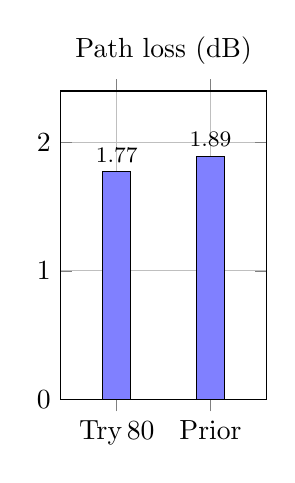
\begin{tikzpicture}
\begin{axis}[barplot, title={Path loss (dB)}, ymax=2.4]
\addplot[fill=blue!50] coordinates {(model,1.77) (prior,1.89)};
\end{axis}
\end{tikzpicture}
\end{minipage}
\hfill
\begin{minipage}{0.31\textwidth}\centering
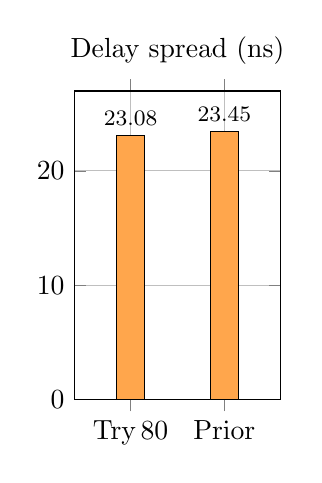
\begin{tikzpicture}
\begin{axis}[barplot, title={Delay spread (ns)}, ymax=27]
\addplot[fill=orange!70] coordinates {(model,23.08) (prior,23.45)};
\end{axis}
\end{tikzpicture}
\end{minipage}
\hfill
\begin{minipage}{0.31\textwidth}\centering
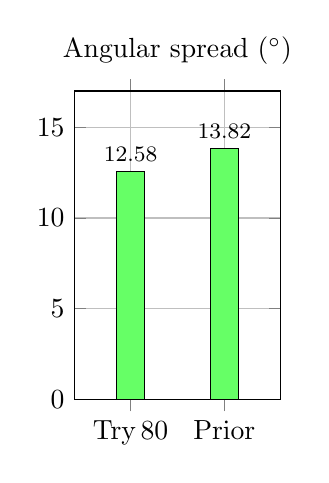
\begin{tikzpicture}
\begin{axis}[barplot, title={Angular spread ($^\circ$)}, ymax=17]
\addplot[fill=green!60] coordinates {(model,12.58) (prior,13.82)};
\end{axis}
\end{tikzpicture}
\end{minipage}
\caption{Current Try 80 validation snapshot against its frozen priors. This
figure is a placeholder until final test evaluation is complete.}
\label{fig:try80_val_placeholder}
\end{figure}

Figure~\ref{fig:try79_panel} shows an example inspection panel from the Try 79
spread-prior analysis. These panels were useful for finding cases where the
calibrated log-domain model worked well and cases where a topology/height
regime needed a fallback.

\begin{figure}[ht]
\centering
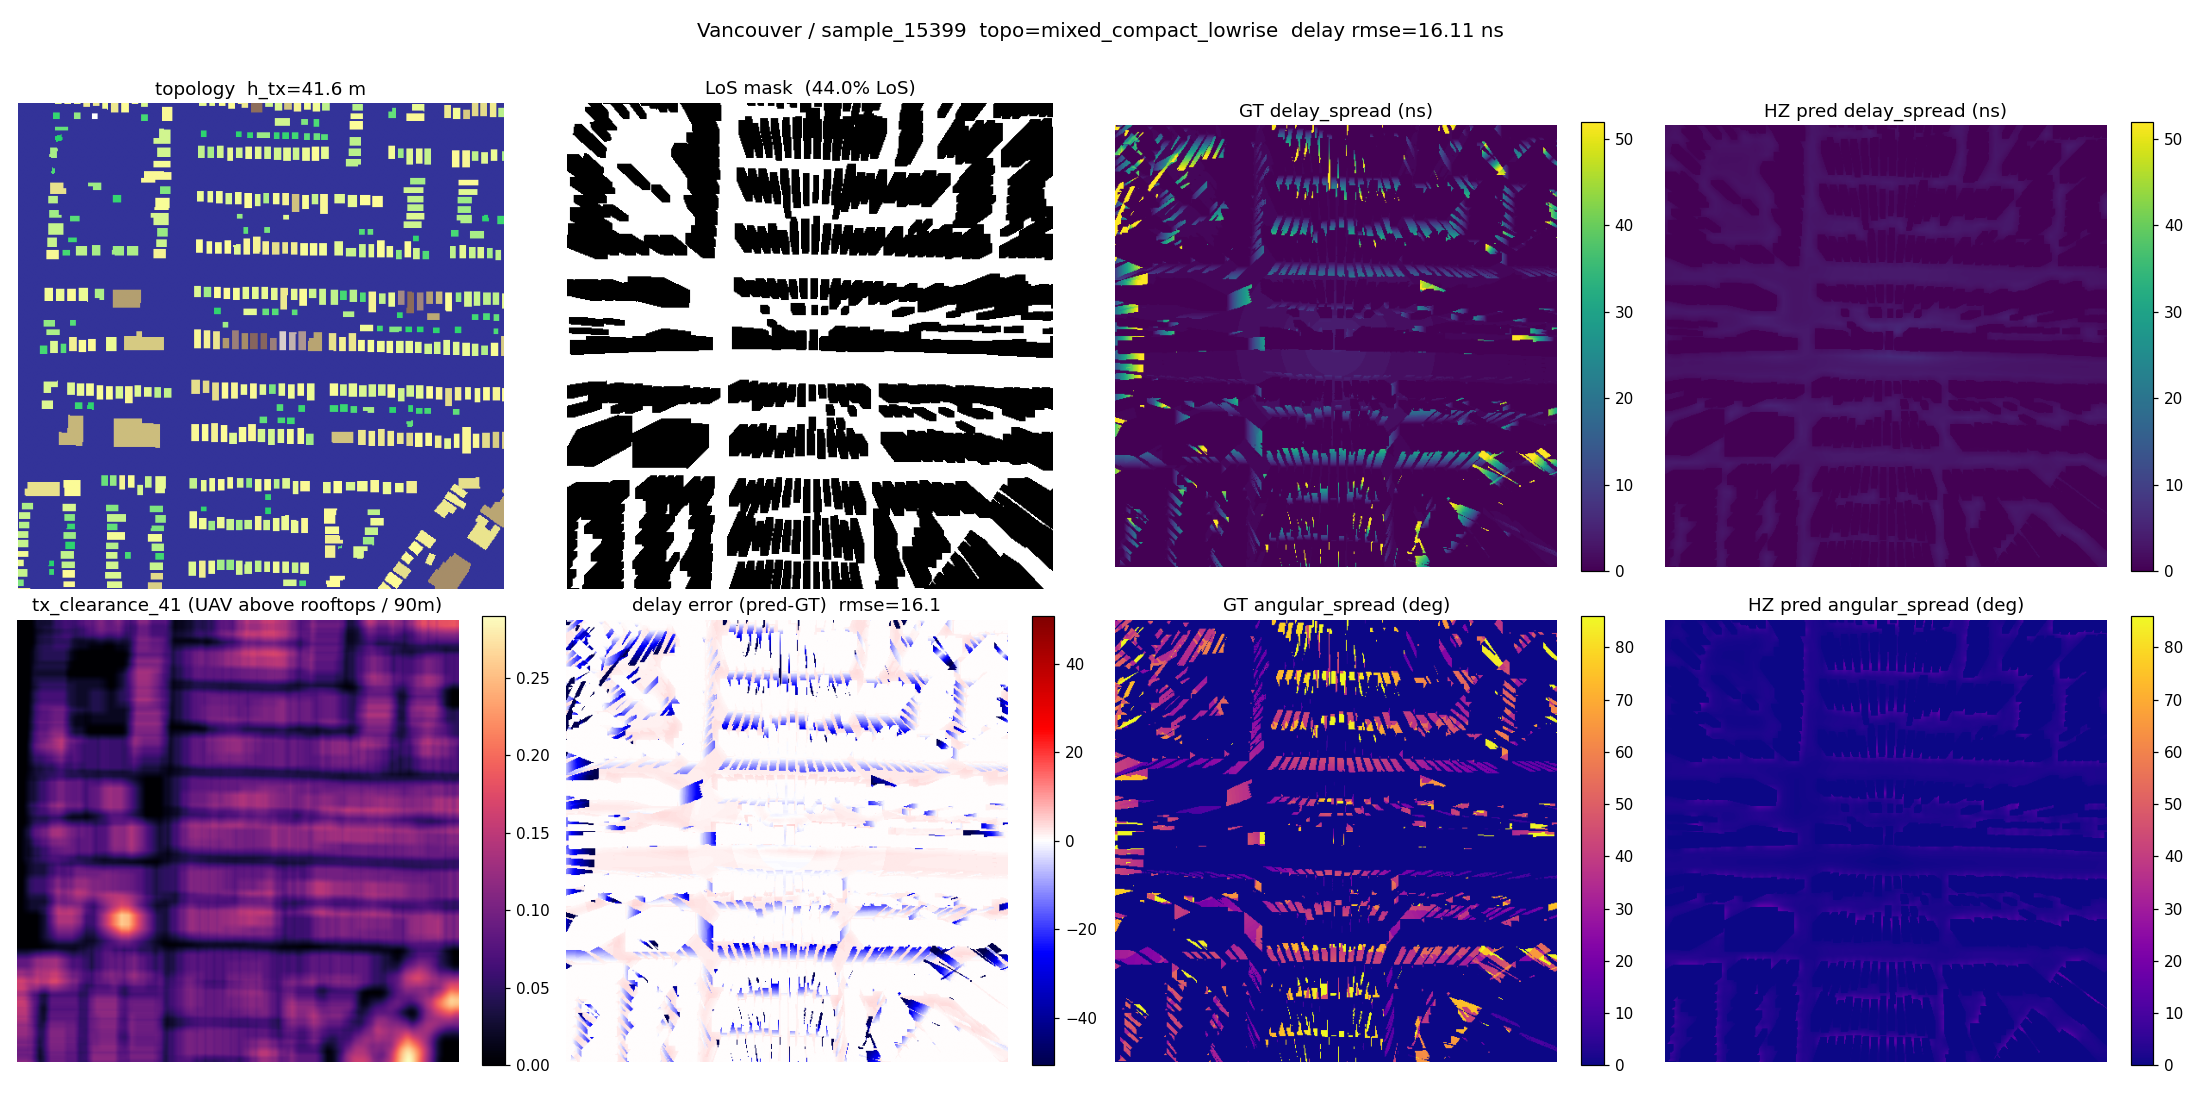
\includegraphics[width=\textwidth]{img/thesis_figures/try79_vancouver_15399_panel.png}
\caption{Example Try 79 inspection panel for a Vancouver sample.}
\label{fig:try79_panel}
\end{figure}

The ongoing Try 80 run also produces a history plot comparing model metrics
against the frozen priors. It is included only as a training diagnostic until
the final checkpoint and test split evaluation are frozen.

\begin{figure}[ht]
\centering
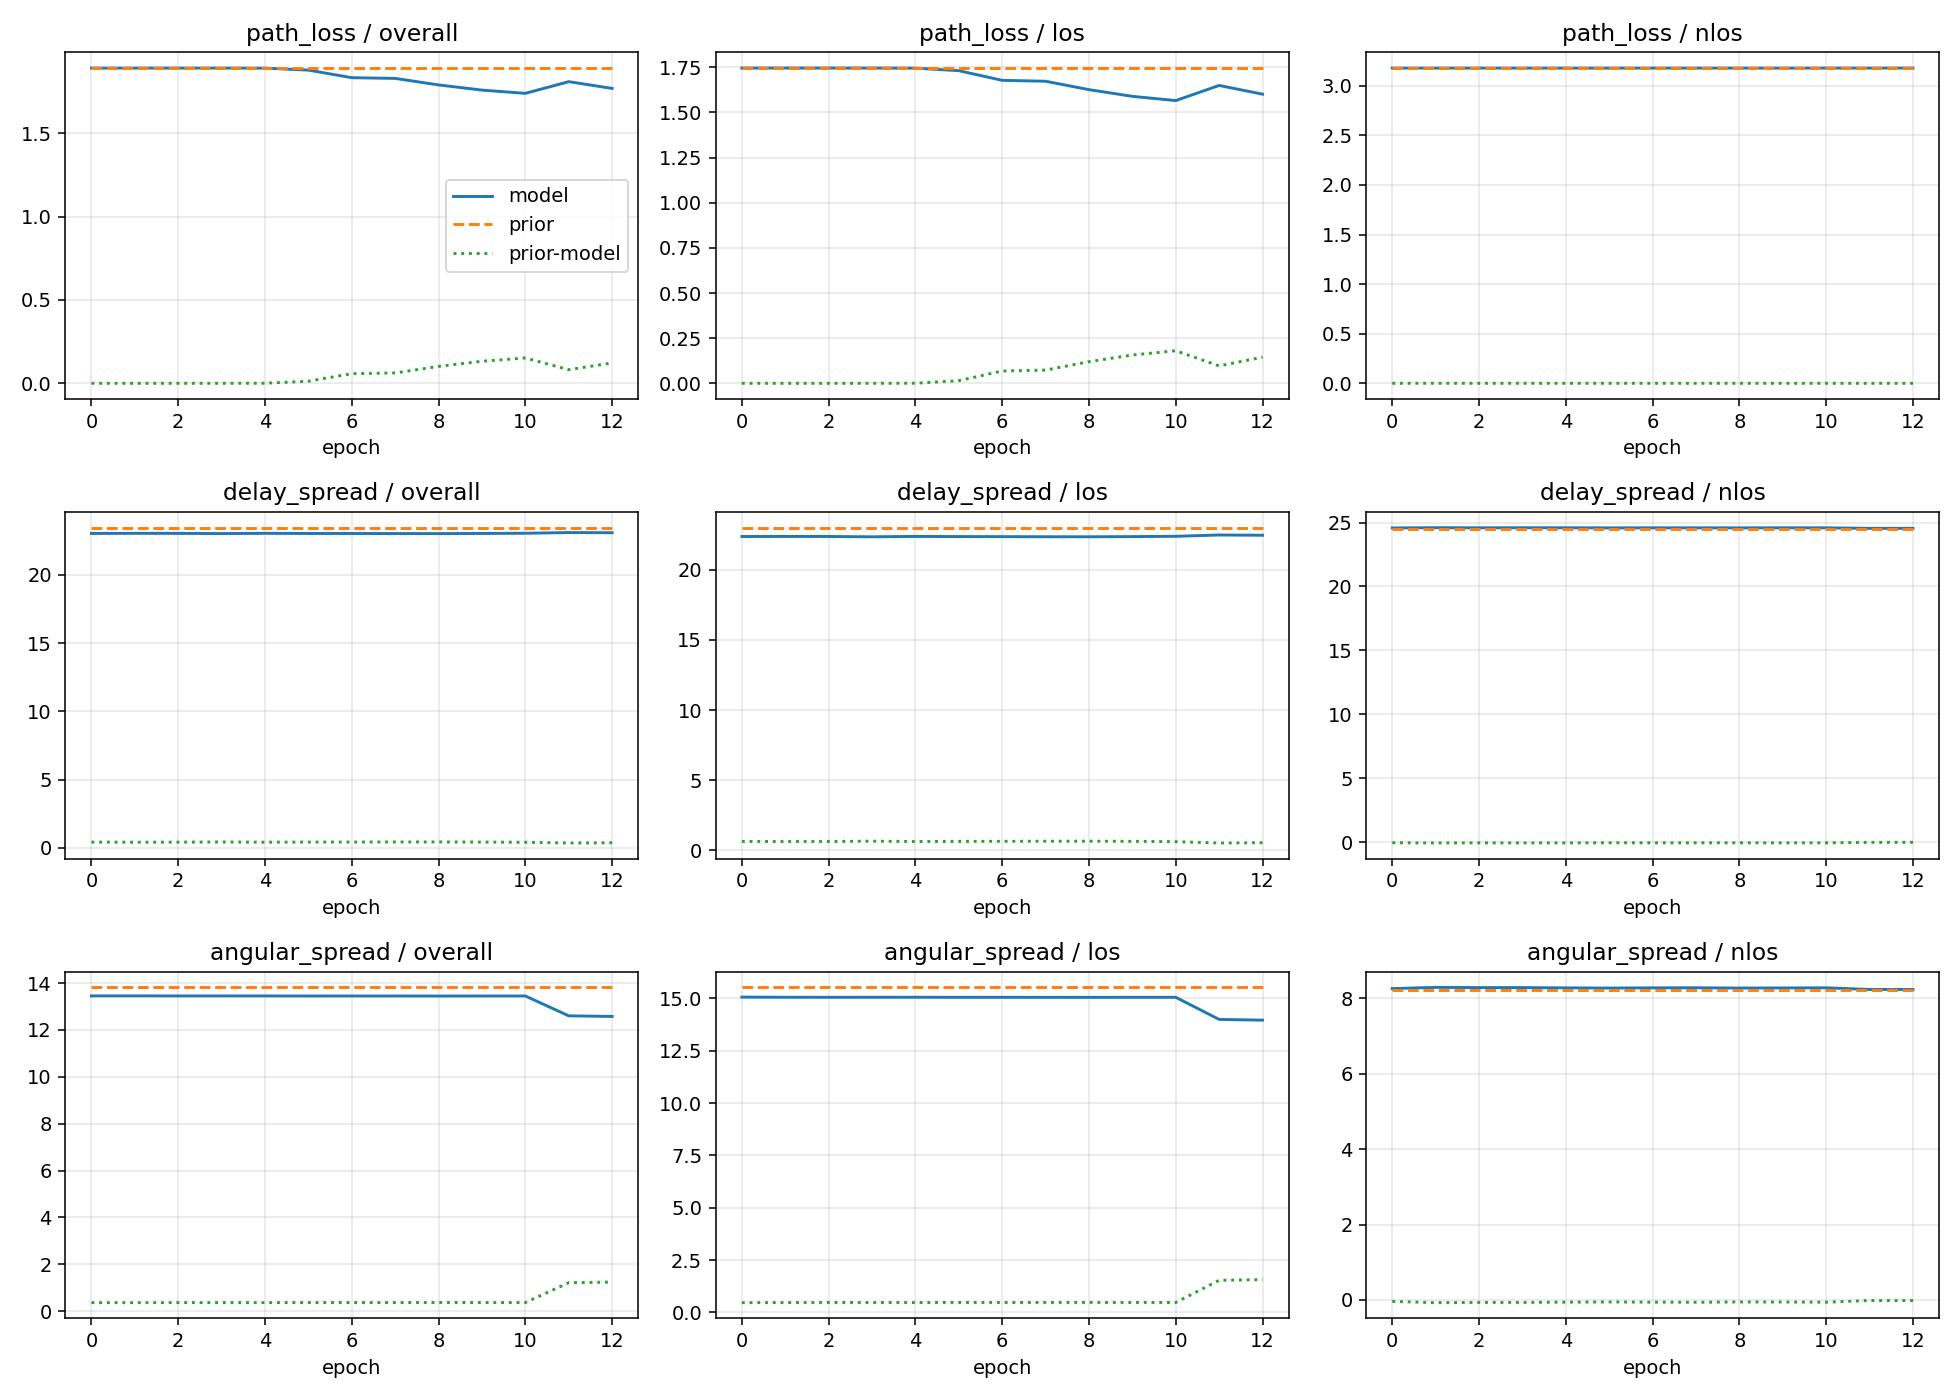
\includegraphics[width=\textwidth]{img/thesis_figures/try80_history_metrics_vs_prior.png}
\caption{Try 80 validation history against frozen priors. Placeholder
diagnostic, not a final test result.}
\label{fig:try80_history}
\end{figure}

The qualitative lesson from Try 78 is equally important: LoS path loss in this
dataset has a strong radial ring structure. Buildings explain visibility and
NLoS morphology, but in LoS they are not the main generator of the residual
shape. This is why a calibrated two-ray model could outperform many neural
iterations that tried to learn the same pattern from pixels alone.

\section{Limitations}

The dataset is produced by ray tracing, not by field measurements. The results
therefore measure agreement with a simulator and not direct over-the-air
deployment performance. The path-loss target is stored as uint8, which imposes
approximately \SI{1}{dB} quantization. The spread targets are also stored as
integer maps: delay spread as uint16 in ns and angular spread as uint8 in
degrees. A more suitable dataset for the final modelling stage would store the
ray-traced targets as float16 or float32 before any display-oriented
quantisation.

The effect can be written explicitly. Let \(y^\star\) be the continuous
ray-traced value and \(y_q = Q_\Delta(y^\star) = y^\star + \epsilon_q\) the
stored value after rounding to step \(\Delta\). Under the usual high-resolution
quantisation approximation, \(\epsilon_q \sim \mathcal{U}(-\Delta/2,\Delta/2)\),
so
\begin{equation}
  \sigma_q = \sqrt{\mathbb{E}[\epsilon_q^2]}
           = \frac{\Delta}{\sqrt{12}}.
  \label{eq:quant_floor}
\end{equation}
With \(\Delta=1\) in the physical units used here, the hidden uncertainty is
\(0.289\,\mathrm{dB}\) for path loss, \(0.289\,\mathrm{ns}\) for delay spread,
and \(0.289^\circ\) for angular spread. This is not the dominant error in the
current Try~80 snapshot, but it is an irreducible resolution limit of the saved
labels and becomes important once residual errors approach the sub-unit regime.

\begin{table}[ht]
\centering
\caption{Approximate quantisation RMSE implied by the stored target precision.
The float16 values use the unit in the upper part of the observed range
(about 180 for path loss/angular spread and 678 for delay spread); float32 is
effectively negligible at this scale.}
\label{tab:quantisation_floor}
\begin{tabular}{lccc}
\toprule
Target & Current integer step & Current floor & Float16 floor near max. \\
\midrule
Path loss & \SI{1}{dB} & \SI{0.289}{dB} & \(\approx\SI{0.036}{dB}\) \\
Delay spread & \SI{1}{ns} & \SI{0.289}{ns} & \(\approx\SI{0.144}{ns}\) \\
Angular spread & \(1^\circ\) & \(0.289^\circ\) & \(\approx0.036^\circ\) \\
\bottomrule
\end{tabular}
\end{table}

This also explains why getting very close to the best possible error is
mathematically harder than the headline RMSE suggests. If model error and
quantisation error are approximately independent, the observed squared error
decomposes as
\[
  \mathbb{E}\!\left[(\hat{y}-y_q)^2\right]
  \approx
  \mathbb{E}\!\left[(\hat{y}-y^\star)^2\right] + \sigma_q^2 .
\]
Near \(\sigma_q\), a real reduction in model error produces only a small change
in total RMSE because of the square-root compression. In addition, many
different continuous ray-tracing values collapse to the same stored integer, so
the model cannot learn sub-bin structure from the labels even if the input
geometry contains enough information. The heavy-tailed NLoS distributions add a
second difficulty: MSE is dominated by rare large misses, so once the common
LoS pixels are near the quantisation scale, further improvements depend on
resolving sparse hard NLoS cases rather than on smoothing the whole map.

The final Try 80 model also still requires a frozen checkpoint and final test
evaluation. The values in Table~\ref{tab:try80_placeholder} are validation
placeholders. They are useful for checking that the joint model is behaving
reasonably, but the final thesis version should replace them with the completed
test split report and the corresponding plots.

Finally, the current dataset fixes frequency and simulator assumptions. A
general outdoor CKM model for deployment would need explicit conditioning on
carrier frequency, bandwidth, antenna pattern, and possibly environment class.
Though that last thing is currently covered by the city-holdout protocol, 
a more flexible model would need to learn to adapt to new environments 
from their geometry rather than just extrapolating from the training cities.
